\documentclass{article}
\usepackage{graphicx} % Required for inserting image
\usepackage{amsmath}
\usepackage{float}
\title{Lesson 6 Homework - Proof Writing}
\author{William Wang}
\date{September 2025}

\begin{document}

\maketitle

\section{}
\begin{figure}[H]
    \centering
    
\includegraphics[width=0.75\linewidth]{q1.png}
    \caption{Graph of the block distance from ceiling over time}
\end{figure}
First we want to find the amplitude and the midline for this function. 
\[\text{Max: } 1.8 \text{, Min: } 1.2 \xrightarrow{} \text{Midline: } \frac{1.8+1.2}{2} = 1.5\]
\[\text{Amplitude} = \frac{1.8-1.2}{2} = 0.3\]
Next we want to find the period
\[\text{Period} = 2*1\text{s} = 2\text{s}\]
Then we have the angular frequency
\[\text{Angular Frequency} = \frac{2\pi}{2} = \pi\]
Then we have the equation of the function
\[f(t) = 1.5+0.3\sin(\pi t+\frac{\pi}{2})\]
Then we can plug in $t = 2.7\text{s}$ into the function
\[f(2.7) = 1.5+0.3\sin(2.7\pi+\frac{\pi}{2}) = 1.32\]
\section{}
\subsection{}
The graph of $y = \sin(x - \frac{\pi}{2})$ is the same as the reflection $y = \cos(x)$ over the $x$ axis. 
\begin{figure}[H]
    \centering
    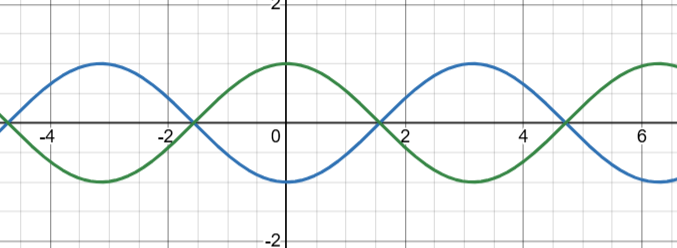
\includegraphics[width=0.75\linewidth]{q2a.png}
    \caption{The graph of the two functions}
\end{figure}
\subsection{}
The graph in the part a suggests that \(f(x) = -g(x)\). This because geometrically on the unit circle, when you subtract \(\frac{\pi}{2}\), you have '
\[\text{Start Coords: } (x_1, y_1) \xrightarrow{} \text{End Coords: } (y_1, -x_1)\]
We have 
\[f(x) = x_1 \text{ and } g(x) = -x_1\]
Hence, we have 
\[f(x) = -g(x)\]
\end{document}
